% begin module tangents-ex2
\begin{frame}
\begin{example}
\begin{columns}[c]
\column{.55\textwidth}
Find an equation for the tangent line to the hyperbola $y = \frac{3}{x}$ at the point $(\alertNoH{2,3,14}{3}, \alertNoH{4,13}{1})$.

\psset{xunit=0.6cm, yunit=0.6cm}
\begin{pspicture}(-5,-3)(5,5)
\psframe*[linecolor=white](-5,-3)(5,5)
\psaxes[ticks=none, labels=none]{<->}(0,0)(-5,-3)(5,5)
\tiny
%Function formula: (3)/(x)
\psplot[linecolor=red, plotpoints=1000]{0.6}{5}{3 x div } %Function formula: (3)/(x)
\psplot[linecolor=red, plotpoints=1000]{-5}{-1}{3 x div }
\rput(2.2, 3){$y=\frac{3}{x}$}

\uncover<16->{
\psline[linecolor=blue](-5, 3.666666667)(5, 0.333333333)
\rput(-2.5, 4){$y=-\frac{x}{3}+2$}
}
\fcFullDot{3}{1}
\rput[t](3, 0.8){\footnotesize $(\alertNoH{2,3,14}{3}, \alertNoH{4,13}{1})$}
\end{pspicture}
%\ \only<handout:0| -8>{%
%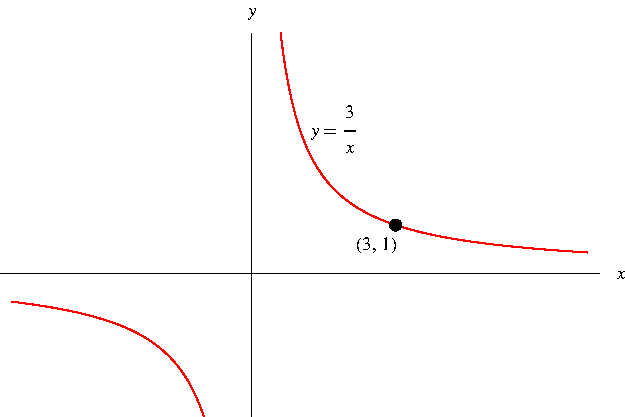
\includegraphics[height=4cm]{derivatives/pictures/03-01-ex2a.pdf}%
%}%
%\only<9->{%
%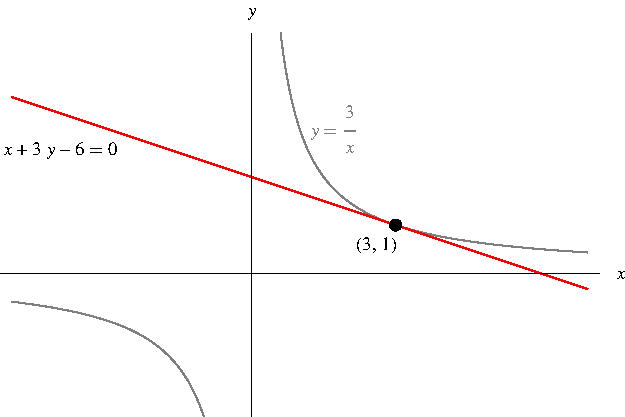
\includegraphics[height=4cm]{derivatives/pictures/03-01-ex2b.pdf}%
%}%

\uncover<13->{
Point-slope form: $y -\alertNoH{13}{1} = \alertNoH{15}{-\frac{1}{3}}(x -\alertNoH{14}{ 3} )$\uncover<16->{, or finally $y = -\frac{x}{3} +2$.}
}
\column{.45\textwidth}
\uncover<2->{%
Here $a = \alertNoH{2,3}{3}$ and $f(\alertNoH{5}{x}) = \frac{3}{\alertNoH{5}{x}}$.
}%
\abovedisplayskip=0pt
\belowdisplayskip=-15pt
\abovedisplayshortskip=0pt
\belowdisplayshortskip=0pt
\begin{align*}
\uncover<3->{\alertNoH{15}{m}} & \uncover<3->{ = }  \uncover<3->{ \lim_{h\rightarrow 0} \frac{f(\alertNoH{5}{\alertNoH{3}{3}+ h})- \alertNoH{4}{ f(\alertNoH{3}{3})}}{h}}\\
& \uncover<4->{ = }  %
\uncover<4->{\lim_{h\rightarrow 0}\frac{\frac{3}{ \alertNoH{5}{3+h}} - \alertNoH{4}{1} }{ h}}\\
& \uncover<6->{ = }  %
\uncover<6->{\lim_{h\rightarrow 0}\frac{\frac{ \alertNoH{7}{3}\alertNoH{7,8}{-}(\alertNoH{7}{3} +\alertNoH{8}{h})}{\alertNoH{9}{ 3+ h} } }{h}}\\
& \uncover<7->{ = }  %
\uncover<7->{\lim_{h\rightarrow 0} \frac{\alertNoH{8}{- \fcCancel{10}{h}} }{ \fcCancel{10}{h} (\alertNoH{9}{3+h})}}\\
& \uncover<10->{ = }  %
\uncover<10->{\alertNoH{11,12}{ \lim_{h \rightarrow 0}-\frac{ 1}{3+h}}} \uncover<11->{\alertNoH{11,12,15}{=}}\fcAnswer{12}{\alertNoH{15}{ -\frac{1}{3}}}
\end{align*}
\end{columns}
\end{example}
\end{frame}
% end module tangents-ex2
